\capitulo{4}{Técnicas y herramientas}

A lo largo del desarrollo del proyecto, se han empleado diversas tecnologías, herramientas y elementos esenciales que requieren familiaridad antes de avanzar en la ejecución del proyecto. La elección de estas opciones en lugar de otras se basa en una evaluación detallada, la cual queda documentada en esta sección con el propósito de brindar una justificación fundamentada.

\section{Entorno Software}
\subsection{Entorno de desarrollo Micropython}\label{4:MicroPython}
%Thonny~\cite{misc:Thonny} 
\begin{itemize}
	\item \textbf{Herramientas valoradas:} \href{https://thonny.org/}{Thonny IDE}, \href{https://codewith.mu/}{Mu Editor}, \href{https://dfrobot.gitbooks.io/upycraft/content/}{Upycraft}, \href{https://www.jetbrains.com/pycharm/}{PyCharm}.
    \item \textbf{Herramienta elegida:} \href{https://thonny.org/}{Thonny IDE}.
\end{itemize}

Thonny IDE se presenta como la opción más idónea, proporcionando una combinación de simplicidad, integración nativa con MicroPython, herramientas de depuración eficaces y un sólido soporte comunitario, todo lo cual contribuye a un entorno de desarrollo eficiente y centrado en el usuario para la programación en la Raspberry Pi Pico W con MicroPython.

\begin{figure}[h]
    \centering
    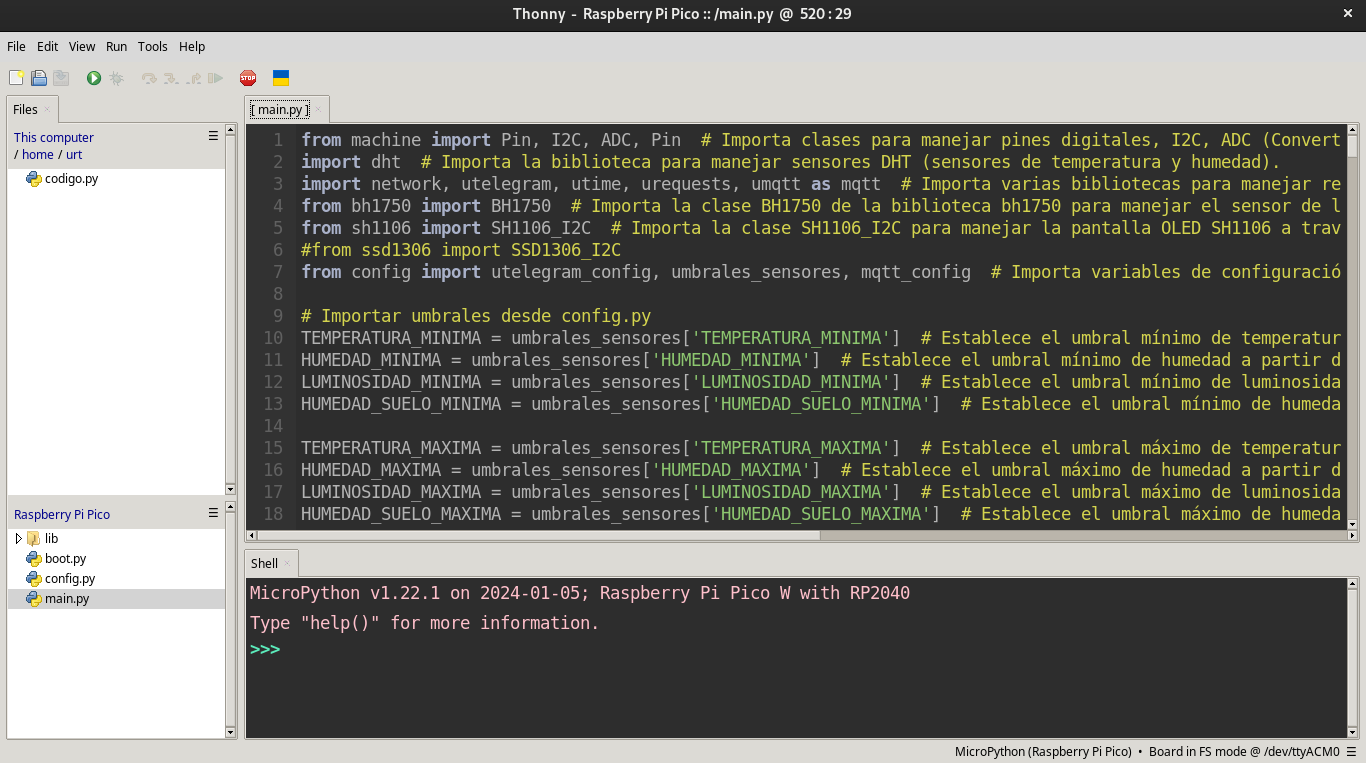
\includegraphics[width=1\textwidth]{img/herramientas/thonny.png}
    \caption{IDE Thonny.} \label{Img:Thonny}
\end{figure}
%Esta parte de la memoria tiene como objetivo presentar las técnicas metodológicas y las herramientas de desarrollo que se han utilizado para llevar a cabo el proyecto. Si se han estudiado diferentes alternativas de metodologías, herramientas, bibliotecas se puede hacer un resumen de los aspectos más destacados de cada alternativa, incluyendo comparativas entre las distintas opciones y una justificación de las elecciones realizadas. 
%No se pretende que este apartado se convierta en un capítulo de un libro dedicado a cada una de las alternativas, sino comentar los aspectos más destacados de cada opción, con un repaso somero a los fundamentos esenciales y referencias bibliográficas para que el lector pueda ampliar su conocimiento sobre el tema.
